\documentclass[a4paper, 12pt]{article}
\usepackage{titling}
\usepackage{array}
\usepackage{booktabs}
\usepackage{enumitem}
\usepackage{graphicx}
\usepackage{hyperref}
\usepackage{amssymb}
\setlength{\heavyrulewidth}{1.5pt}
\setlength{\abovetopsep}{4pt}
\graphicspath{{.}}

\usepackage[margin=1in]{geometry}

% Must be after geometry
\usepackage{fancyhdr}
\pagestyle{fancy}
\fancyhf{}
\rhead{NN Homework 1}
\lhead{P.Lukin, I. Vishniakou, E. Ovchinnikova}
\cfoot{\thepage}

\setlength{\droptitle}{-5em}

\title{Neural Networks  \\
				- Homework 1 -}
\author{Petr Lukin, Ivan Vishniakou, Evgeniya Ovchinnikova}
\date{Lecture date: 26 September 2016}

\begin{document}

\maketitle

\section{Mind map}
Neural network (NN) is a parallel distributed system consisted of computing cells ("neurons") that is capable of storing and using experimental knowledge to model a brain in processes of certain tasks performance.

\begin{figure}[h]
  \centering
  \caption{S. Haykin, Neural Networks, chapter 1. Mind map (a zoomed version of the map is attached as NN.png file).\label{fig:mindMap}}
  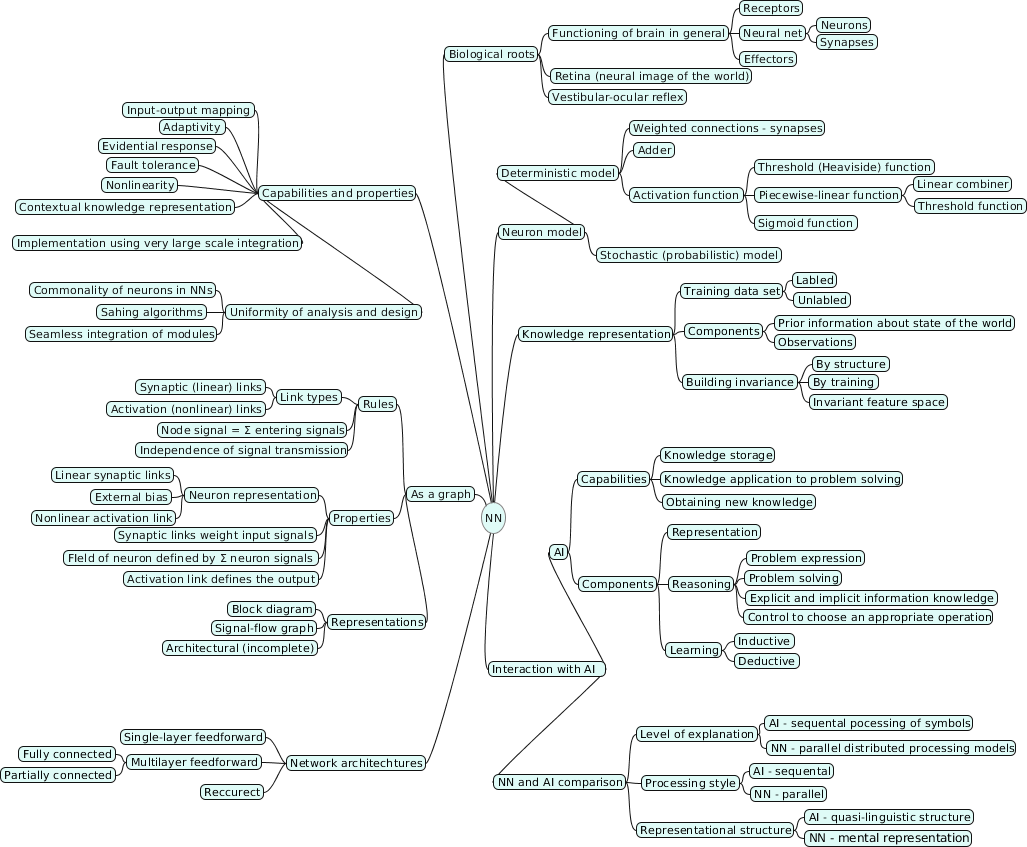
\includegraphics[width=1.0\textwidth]{NN}
\end{figure}



\end{document}
